\section{AI-Assisted Authoring Workflow}
\label{sec:authoring-workflow}

\begin{figure}
    \centering
    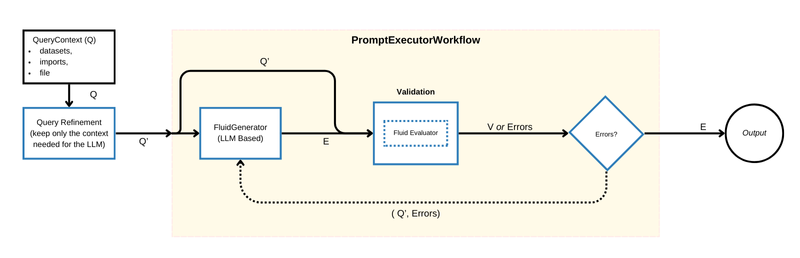
\includegraphics[width=0.95\linewidth]{fig/authoring-assistant-architecture.png}
    \caption{AI-assisted authoring workflow}\label{fig:architecture}
\end{figure}

\subsection{System Prompt}
\label{subsec:system-prompt}
Fig. \ref{fig:system-prompt} shows the system prompt defined for the Authoring Assistant.

\begin{figure}[h]
    \centering
    \begin{tcolorbox}[colback=gray!10, colframe=gray!50, boxrule=0.5pt, arc=2pt,
        left=6pt, right=6pt, top=4pt, bottom=4pt]
        \VerbatimInput[fontsize=\small, formatcom=\normalfont]{system-prompt/system-prompt.txt}
    \end{tcolorbox}
    \vspace{-0.5em}
    \caption{System-Prompt defined for the Authoring Assistant}
    \label{fig:system-prompt}
\end{figure}


\subsection{Editor Loop}
\label{subsec:editor-loop}
Design of main loop that would be integrated into an IDE. The configuration (state) that is being maintained
is a \kw{Paragraph} the user is authoring in Fluid. Consists of a sequence of text fragments, some of which
are uninterpreted (plain literals), the remainder have underlying expressions linking the text to raw or derived
data.

Workflow:
\begin{enumerate}
\item User selects (a substring of) one of the literal text fragments, indicating they want to link it in this
way
\item Authoring tool generates expression which is either:
  \begin{enumerate}
  \item computes the selected text (e.g.~``greater than'' might be computed by comparing two numbers)
  \item becomes the formal meaning of the selected text (e.g. the text ``carbon intensity of methane
emissions'' can be understood in a specific context as referring to the numerical value ``34 gCO2eq/kWh''
  \end{enumerate}
\item Some kind of validation step, including both automated validation (e.g. checking for runtime errors) and
user validation; if validation fails, goto (2)
\item Partition code into additional definitions and expression; add definitions to main source file, and
incorporate expression into \kw{Paragraph}
\item Goto (1) with updated editor state
\end{enumerate}

\subsection{Loopback System}
\label{subsec:loopback-system}

Once the Authoring Assistant has generated the expression, it is executed by the Fluid interpreter.
If execution fails, the error is sent back to the LLM for regeneration.
This \textit{loopback} mechanism enables iterative refinement of expressions, improving accuracy and robustness.
Three types of errors are handled:

\begin{itemize}
    \item \textbf{Invalid Program}.
    The generated expression is executed by the Fluid interpreter.
    If the execution fails due to issues such as undeclared functions, syntax errors, or other interpreter-level problems, it results in an \textit{Invalid Program} error.
    \item \textbf{Invalid Output Type}.
    According to the \textit{System Prompt} (Fig.~\ref{fig:system-prompt}), the expression is expected to return a string value.
    If the returned value is of a different type, an \textit{Invalid Output Type} error is raised.
    \item \textbf{Invalid Output Value}.
    The output produced by the generated expression is compared against the highlighted target text.
    If the values do not match, an \textit{Invalid Output Value} error is reported.
\end{itemize}

\subsection{Paragraph with generated expression}
\label{subsec:paragraph-with-generated-expression}
Figure \ref{fig:fluid-example-paragraph} shows the Fluid code of a Paragraph with the expression generated by the authoring assistant.
Figure \ref{fig:fluid-scigen} shows the Fluid code written for the scigen datasets and examples.
\begin{figure}[h]
    \small
    {\lstinputlisting[language=Fluid]{website/authoring-assistant/fluid/1805.02474v1-10.fld}}
    \vspace{-0.5em}
    \caption{Fluid source code example Paragraph}
    \label{fig:fluid-example-paragraph}
\end{figure}

\begin{figure}[h]
    \small
    {\lstinputlisting[language=Fluid]{fluid-common/scigen.fld}}
    \vspace{-0.5em}
    \caption{Fluid library written for scigen}
    \label{fig:fluid-scigen}
\end{figure}

\subsection{Turning validation errors into improved prompts}\label{subsec:turning-validation-errors-into-improved-prompts}
E.g.:
\begin{enumerate}
\item Turn ``Definition not found'' into prompt to generate definition?
\end{enumerate}

\subsection{IDE integration}\label{subsec:ide-integration}

Could then be integrated into desktop IDE like VSCode or online IDE like CodeMirror. Might make a good
internship project, but could also be out-of-scope for this paper.

\subsection{Other potential enhancements}\label{subsec:other-potential-enhancements}

We could also think about using an LLM in a couple of other complementary ways:
\begin{itemize}
\item identifying text fragments which might be linked;
\item validating generated expressions (perhaps by proposing test cases)
\end{itemize}


